\documentclass[11pt]{article}
\newcommand\Decide[1]{#1}
\makeatletter
\def\sectionsuffix      {}
\def\subsectionsuffix   {\quad}
\def\subsubsectionsuffix{\quad}
\def\paragraphsuffix    {\quad}
\renewcommand\@seccntformat[1]{\csname the#1\endcsname\csname#1suffix\endcsname}
\renewcommand\thesection{\protect\Decide{\@arabic\c@section}}
\renewcommand\thesubsection{\@arabic\c@section.\@arabic\c@subsection}
\makeatother

\usepackage{tabularx}
\usepackage[none]{hyphenat}
\usepackage[utf8x]{inputenc}
\usepackage{lmodern,textcomp}
\usepackage{enumitem}
\usepackage{ltablex}
\usepackage[english]{babel}
\usepackage{blindtext}
\usepackage{microtype}
\usepackage[hidelinks]{hyperref}
\usepackage{hanging}
\usepackage[paperheight=279.4mm,paperwidth=210mm,bottom=10em]{geometry}
\usepackage[final]{pdfpages}
\usepackage{tocloft}
\usepackage{hyperref}
\usepackage{setspace}
\usepackage[bottom]{footmisc}
\usepackage{graphicx}
\usepackage{subcaption}

\setlength\cftparskip{0pt}
\setlength\cftbeforesecskip{0pt}

\usepackage{fancyhdr}
\setlength{\parskip}{1em}
\setlength\cftparskip{5pt}
\setlength\cftbeforesecskip{5pt}
\setlength\cftaftertoctitleskip{10pt}

\setlist[itemize]{leftmargin=*}

\usepackage{titlesec}

\titlespacing\chapter{0pt}{12pt}{-5pt}
\titlespacing\section{0pt}{12pt plus 2pt minus 2pt}{-5pt plus 2pt minus 2pt}
\titlespacing\subsection{0pt}{12pt plus 2pt minus 2pt}{-5pt plus 2pt minus 2pt}
\titlespacing\subsubsection{0pt}{12pt plus 2pt minus 2pt}{-5pt plus 2pt minus 2pt}

\pagestyle{fancy}
\fancyhf{}
\fancyhead[LE,RO]{\iffloatpage{}{Teaching Statement}}
\fancyhead[RE,LO]{\iffloatpage{}{Anthony Kevins}}
\fancyfoot[CE,CO]{\thepage}
\setlength\parindent{0pt}
\setlist[itemize]{leftmargin=*}

\begin{document}

	\section{ Teaching Philosophy, Strategies, and Goals}

	My teaching is shaped by the belief that a political science education has the potential to help form not only good political scientists, but also good citizens. In an age in which formulaic talking points often pass for quality political discourse, I believe that political science can help students move beyond facile arguments by improving their substantive political knowledge, scientific literacy, and critical reasoning skills. As a teacher, my task is to facilitate this growth by encouraging students to actively engage with both the course material and their peers. I do so by employing pedagogical best-practices tied to constructive alignment, active learning, and an open dialogue with students.

	My course development centres around the notion that intended learning outcomes, active learning activities, and student assessment tasks should all be closely aligned (i.e. constructive alignment). The first step in this process is the careful defining of learning objectives. Outlining these goals helps to maintain consistency across the course materials and assessment methods, while also ensuring that students are familiar with the skills they are meant to develop. For example, in \textit{Political Institutions}, an undergraduate core course that I co-developed and co-taught, the compendium laid out the learning objectives for the course as a whole and for each of the individual weeks (see \hyperref[sec:compendium]{Section 3.1}). By specifying in advance not only every lecture's theoretical and empirical objectives, but also the corresponding tutorial's theory-application objectives, we were able to ensure a clear thread throughout the semester. 

	Having identified learning goals, I then develop individual lesson plans that allow me to build toward the intended learning outcomes in an engaging way. In a master's-level seminar course on \textit{Democracy and Representation}  (see \hyperref[sec:syllabus]{Section 3.2}), for example, I opened each class with a brief discussion of a contemporary political issue connected to the lesson's topic (e.g., discussing British newspaper coverage of Jeremy Corbyn in a lesson looking at the media's role in shaping public opinion). Two goals guided this introductory framing: first, to tie the readings to current events and controversies, thereby highlighting the practical relevance of the course material; and second, to set the stage for theory-application later in the lesson, ensuring students have weekly opportunities to apply theories from the curriculum to real-world cases. 

	Because this higher-level engagement requires a strong grasp of the assigned material, my lesson planning is also attuned to assuring student understanding. After connecting the week's topic to contemporary events or debates, I lay out a road map for the class by providing a set of questions they should be able to answer by the end of the day's session. I revisit key concepts over the course of the lesson through a combination of lecturing and active learning activities, having students, typically in pairs or small groups, engage with questions of understanding. These latter activities have taken a variety of formats, including online quizzes (followed by peer and then class-wide discussions), flipped classroom activities where students do the teaching, and reflections on the ``muddiest'' point of the lesson. These techniques allow me to ascertain how well students have grasped the course material while at the same time encouraging peer-to-peer explanation -- which, in turn, helps to facilitate active learning and overcome some of the difficulties inherent in the instructor-student knowledge gap.

	Once students have a reasonable grasp of the material, I move on to more advanced learning objectives. While these goals vary based on the level and subject of a given course, this deeper exploration of a topic often involves several steps: applying an argument or theory to an event or case; analyzing the case from an alternative framework; and using the Socratic method to have students reflect upon any underlying assumptions. Furthermore, in-class discussions and debates are complemented by a variety of pre-class activities, including the preparation of small written assignments, group presentations, or methods exercises (with the aid of original screencasts for more technical tasks). These exercises help students to cement comprehension and refine the research, presentation, and writing skills that they will need after graduation.

	My course design also incorporates various larger learning activities that punctuate the semester, with the aim of consolidating the skills and knowledge developed in individual lessons. In addition to the traditional graded assessments, my courses have included periodic stats labs, review sessions, and writing workshops. Some of these activities clearly necessitate more teacher intervention than others, but I always ensure that peer feedback plays a central role. In having students assist and assess one another, I seek to: (1) equip them with tools to more critically evaluate their own work; and (2) help them to develop skills that align with the course's learning objectives and the associated assessment tasks. At the same time, this approach also generates more frequent feedback for students and a more participatory classroom dynamic.

	The final defining feature of my pedagogical approach is an open dialogue with students. Achieving this dialogue involves expressly making the case for the teaching activities I employ and then offering students the chance to provide informal, anonymous feedback after the first month of the semester. In my experience, this back-and-forth typically engenders a greater openness to new activities on their part. For example, some students have initially expressed doubt that peer feedback could be useful, based on the belief that only comments from their eventual grader are important; yet I have found that if I explain the motivations for this approach in advance, they quickly come to recognize and appreciate its benefits. The corollary of this, however, is that I must demonstrate an honest openness to adapting my teaching and learning activities when students are left unconvinced or have suggestions for improvements. 

	Overall, my teaching practices are grounded in two beliefs: that a strong political science education can provide tools to make us better citizens; and that advances in pedagogical research can help us to more effectively reach our teaching goals. I look forward to a career in which I continually improve my ability to teach and engage students, building from their feedback while experimenting with new pedagogical techniques.\\[-5ex]


	\section{ Teaching Experience and Training}

	My teaching experience includes undergraduate and graduate course development and instruction, in formats ranging from small seminars to large lectures involving several hundred students. I have taught both methodological and substantive subject matter, covering topics in Comparative Politics, Political Behaviour, International Relations, and Research Methods.

	The syllabi for three of these courses (marked with asterisks) are provided at the end of this teaching statement, alongside evaluations of my teaching.\\[-5ex]

	\begin{itemize}[noitemsep]
		\item \textbf{Co-Instructor, “Political Institutions: Western countries, The European Union and International Institutions”*}\\[-4ex]
		\begin{itemize}[noitemsep]
			\item \textbf{Overview}: Bachelor’s Core Course, Aarhus University, Spring 2016 \& 2017 (Enrolment: 311 \& 317)
			\item \textbf{Duties}: Course design, lectures, exam design, and weekly seminars
        	\item \textbf{In-Class Teaching Time}: Approximately 94 hours (per semester)
			\item \textbf{Course Description}: A survey course on institutionalism and various domestic and supranational institutions, with a particular focus on the EU
			\item \textbf{Sample Topics}: Electoral Systems and Party Systems; Federalism; Executive Politics in the EU.
		\end{itemize}
		\item \textbf{Co-Instructor, “Social Science Methods for Journalists”}\\[-4ex]
		\begin{itemize}[noitemsep]
			\item \textbf{Overview}: Master’s Core Course, Aarhus University, Fall 2016 (Enrolment: 80)
			\item \textbf{Duties}: Course design, lectures, exam design, grading, and weekly seminars
          	\item \textbf{In-Class Teaching Time}: Approximately 30 hours
			\item \textbf{Course Description}: An introduction to social science research design and methods (both quantitative and qualitative)
			\item \textbf{Sample Topics}: Case Selection and Data Sampling; Designing and Conducting Interviews and Surveys; Introduction to Statistical Inference.
		\end{itemize}
		\item \textbf{Instructor, “Democracy and Representation”*}\\[-4ex]
		\begin{itemize}[noitemsep]
			\item \textbf{Overview}: Master’s Seminar, Aarhus University, Fall 2015 (Enrolment: 11)
			\item \textbf{Duties}: Course design, instruction, exam design, and grading
    	    \item \textbf{In-Class Teaching Time}: Approximately 45 hours
			\item \textbf{Course Description}: An exploration of the bi-directional link between public opinion and policy making, including patterns of unequal representation
			\item \textbf{Sample Topics}: The Survey Method; Uses and Abuses of Public Opinion Data; Democracy in the European Union.
		\end{itemize}
		\item \textbf{Instructor, “Pragmatism and Politics”}\\[-4ex]
		\begin{itemize}[noitemsep]
			\item \textbf{Overview}: Master’s Seminar, Aarhus University, Spring 2015 (Enrolment: 4)
			\item \textbf{Duties}: Course design, instruction, exam design, and grading
        	\item \textbf{In-Class Teaching Time}: Approximately 45 hours
			\item \textbf{Course Description}: An examination of the challenges underlying the balance between technocracy and democracy
			\item \textbf{Sample Topics}: The End of Ideology; Philosophical versus Everyday Pragmatism; A Democratic Deficit?
		\end{itemize}
		\item \textbf{Instructor, “Politics: Contemporary Europe”}\\[-4ex]
		\begin{itemize}[noitemsep]
			\item \textbf{Overview}: Bachelor’s Course, McGill University, Summer \& Fall 2013 (Enrolment: 34 \& 75)
			\item \textbf{Duties}: Course design, lectures, exam design, and grading
        	\item \textbf{In-Class Teaching Time}: Approximately 38 hours (per semester)
			\item \textbf{Course Description}: A survey of welfare state, capitalist, and citizenship regime typologies, as well as the policy changes across them
			\item \textbf{Sample Topics}: Towards a Two-Tiered Welfare State?; Is European Capitalism Different?; How do Different Types of Nationalism Affect Tolerance? \\[-5ex]
		\end{itemize}
	\end{itemize} 

	This classroom experience is complemented by considerable formal pedagogical training. In addition to various short workshops on topics such as blended learning, effective lecturing, and the use of active learning in large-class settings, I participated in the following formal pedagogical courses from Aarhus University’s Centre for Teaching and Learning:\\[-5ex]

	\begin{itemize}[noitemsep]
		\item Teacher Training Programme for Assistant Professors, 2016-2017
		\begin{itemize}[noitemsep]
			\item	This (5 ECTS) programme consisted of a three-day residential course as well as three subsequent full-day workshops
			\item Topics included Teaching Methods and Organization, Integrated Course Design, Lecturing Skills, and Educational IT
		\end{itemize}
		\item Challenges of the Multicultural Classroom in a Danish Context, 2016
		\begin{itemize}[noitemsep]
			\item This course consisted of a four-hour workshop on the Danish pedagogical approach to seminar-based teaching and an hour-long evaluation of each participant's teaching\\[-5ex]
		\end{itemize}
	\end{itemize}

\smallskip

\section{ Documentation of Teaching Excellence}

The remainder of this document contains evidence of my teaching competencies. This includes: the compendium for a bachelor's core course that I co-developed and co-taught (\hyperref[sec:compendium]{Section 3.1}); a syllabus from one of my graduate seminars (\hyperref[sec:syllabus]{Section 3.2}); a syllabus for a mixed methods master's core course that I co-taught (\hyperref[sec:methods]{Section 3.3}); a letter of feedback from Ole Lauridsen (Deputy Director of Aarhus University’s Centre for Teaching and Learning), provided after he sat in on one of my classes as part of a pedagogical course (\hyperref[sec:letter]{Section 3.4}); and a varied selection of student evaluations from my courses (\hyperref[sec:evals]{Section 3.5}), listed here in chronological order (please note that a few of the student comments are written in Danish).

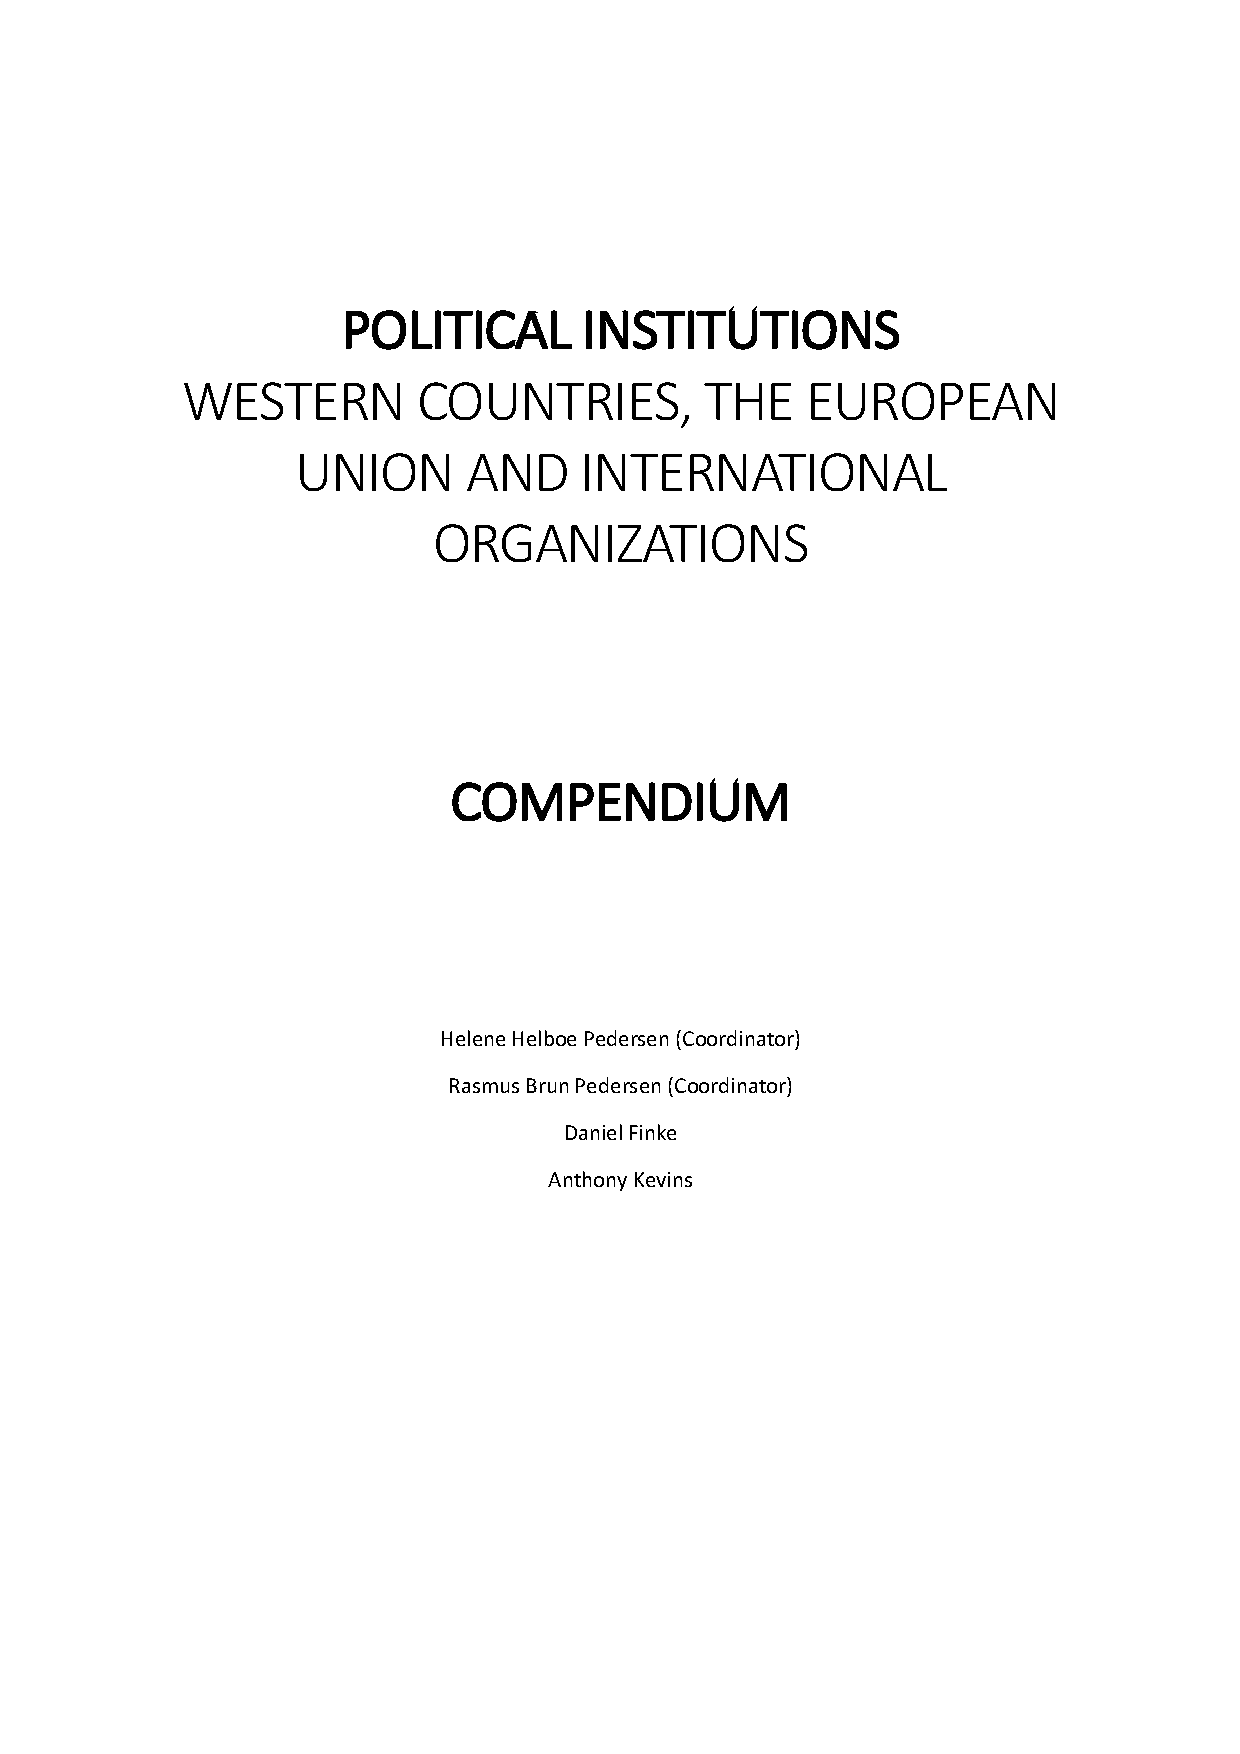
\includepdf[pages=1,pagecommand={\thispagestyle{plain}\subsection{Undergraduate Course Compendium}\label{sec:compendium}},
height=\textheight,keepaspectratio,trim=80pt 80pt 80pt 80pt]{Undergraduate.pdf}
\includepdf[pages=2-21,pagecommand={\thispagestyle{plain}},height=\textheight,keepaspectratio,trim=80pt 80pt 80pt 80pt]{Undergraduate.pdf}
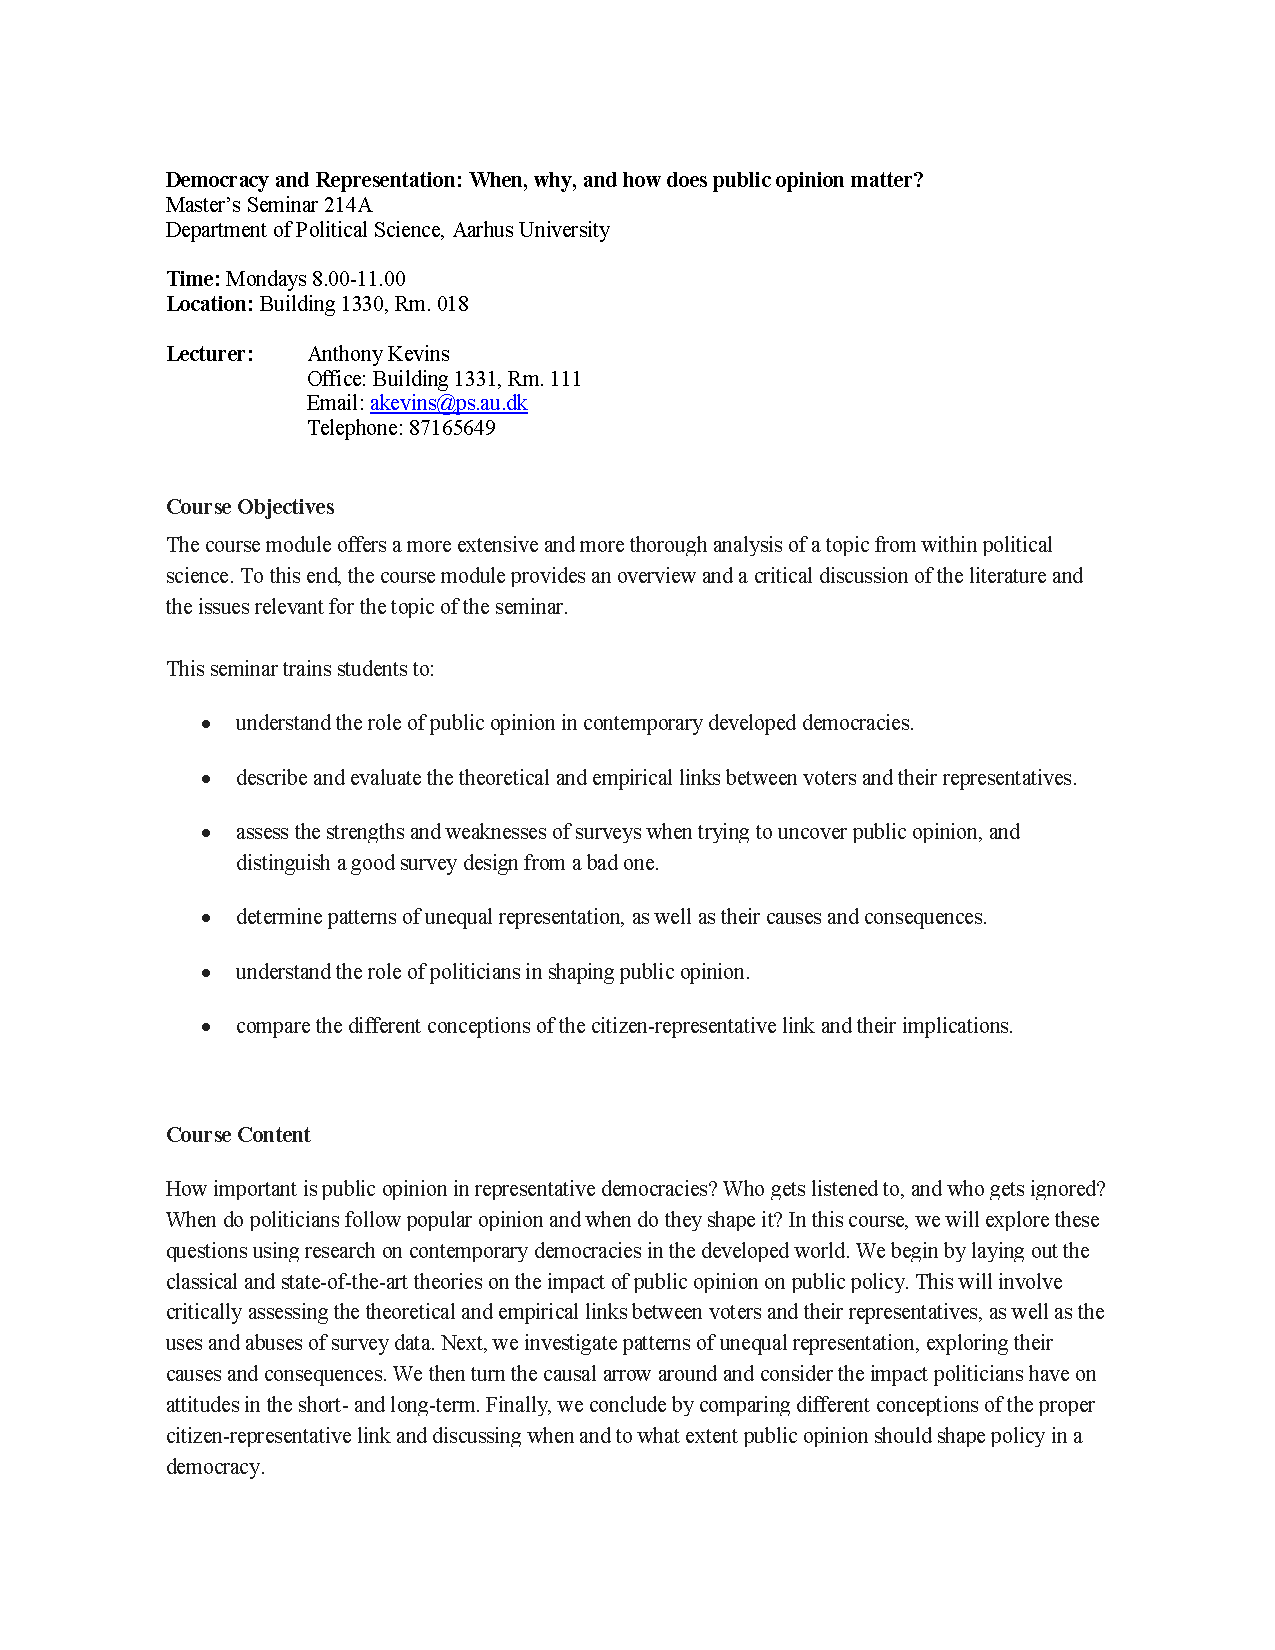
\includepdf[pages=1,pagecommand={\thispagestyle{plain}\subsection{Graduate Seminar Syllabus}\label{sec:syllabus}},height=\textheight,keepaspectratio,trim=60pt 60pt 60pt 60pt]{Graduate.pdf}
\includepdf[pages=2-7,pagecommand={\thispagestyle{plain}},height=\textheight,keepaspectratio,trim=60pt 60pt 60pt 60pt]{Graduate.pdf}
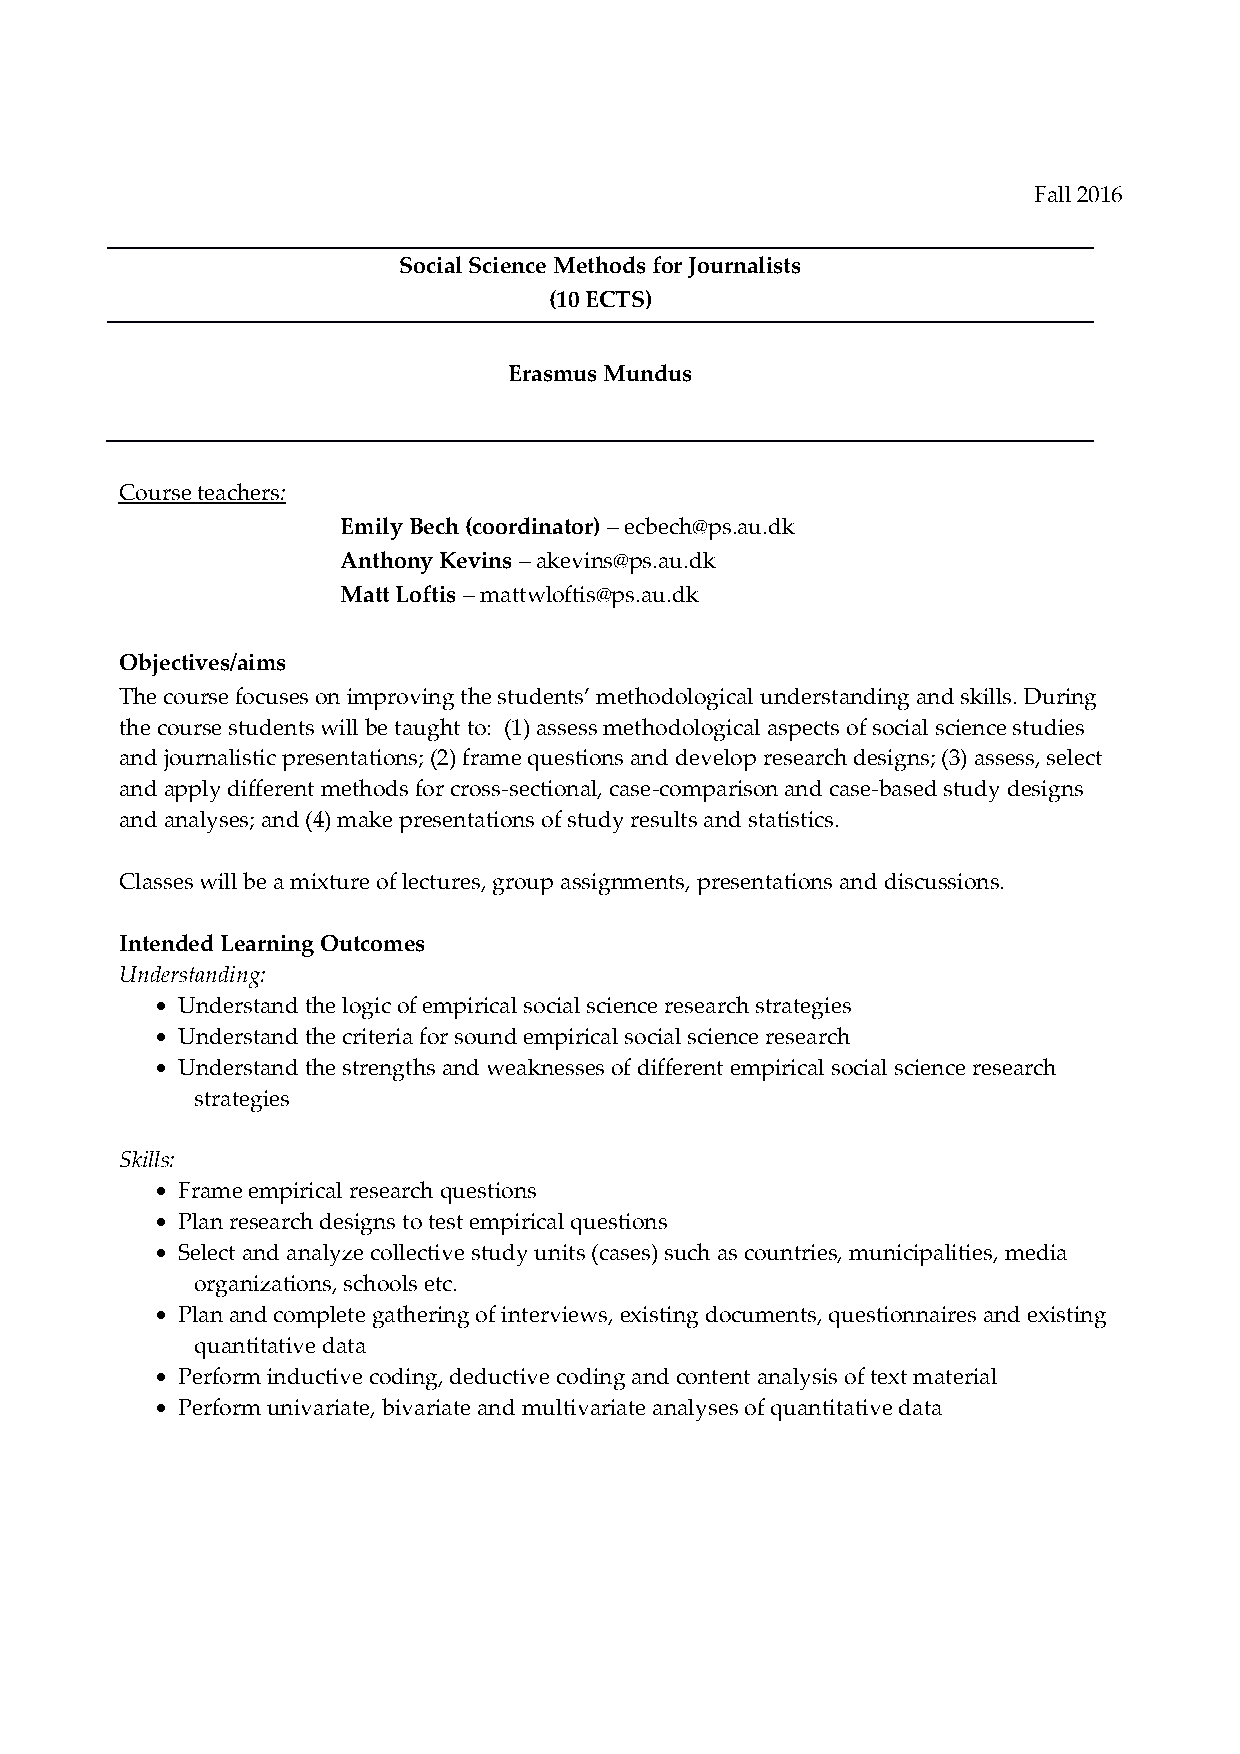
\includepdf[pages=1,pagecommand={\thispagestyle{plain}\subsection{Methods Course Syllabus}\label{sec:methods}},height=\textheight,keepaspectratio,trim=60pt 60pt 60pt 60pt]{Methods.pdf}
\includepdf[pages=2-14,pagecommand={\thispagestyle{plain}},height=\textheight,keepaspectratio,trim=60pt 60pt 60pt 60pt]{Methods.pdf}

\includepdf[pages=36,pagecommand={\thispagestyle{plain}\subsection{Teaching Supervision Feedback}\label{sec:letter}},height=\textheight,keepaspectratio,trim=50pt 50pt 50pt 50pt]{Appendix_Materials.pdf}

\includepdf[pages=37,pagecommand={\thispagestyle{plain}\subsection{Student Evaluations}\label{sec:evals}},width=\textwidth,height=\textheight,keepaspectratio,trim=30pt 30pt 30pt 30pt]{Appendix_Materials.pdf}
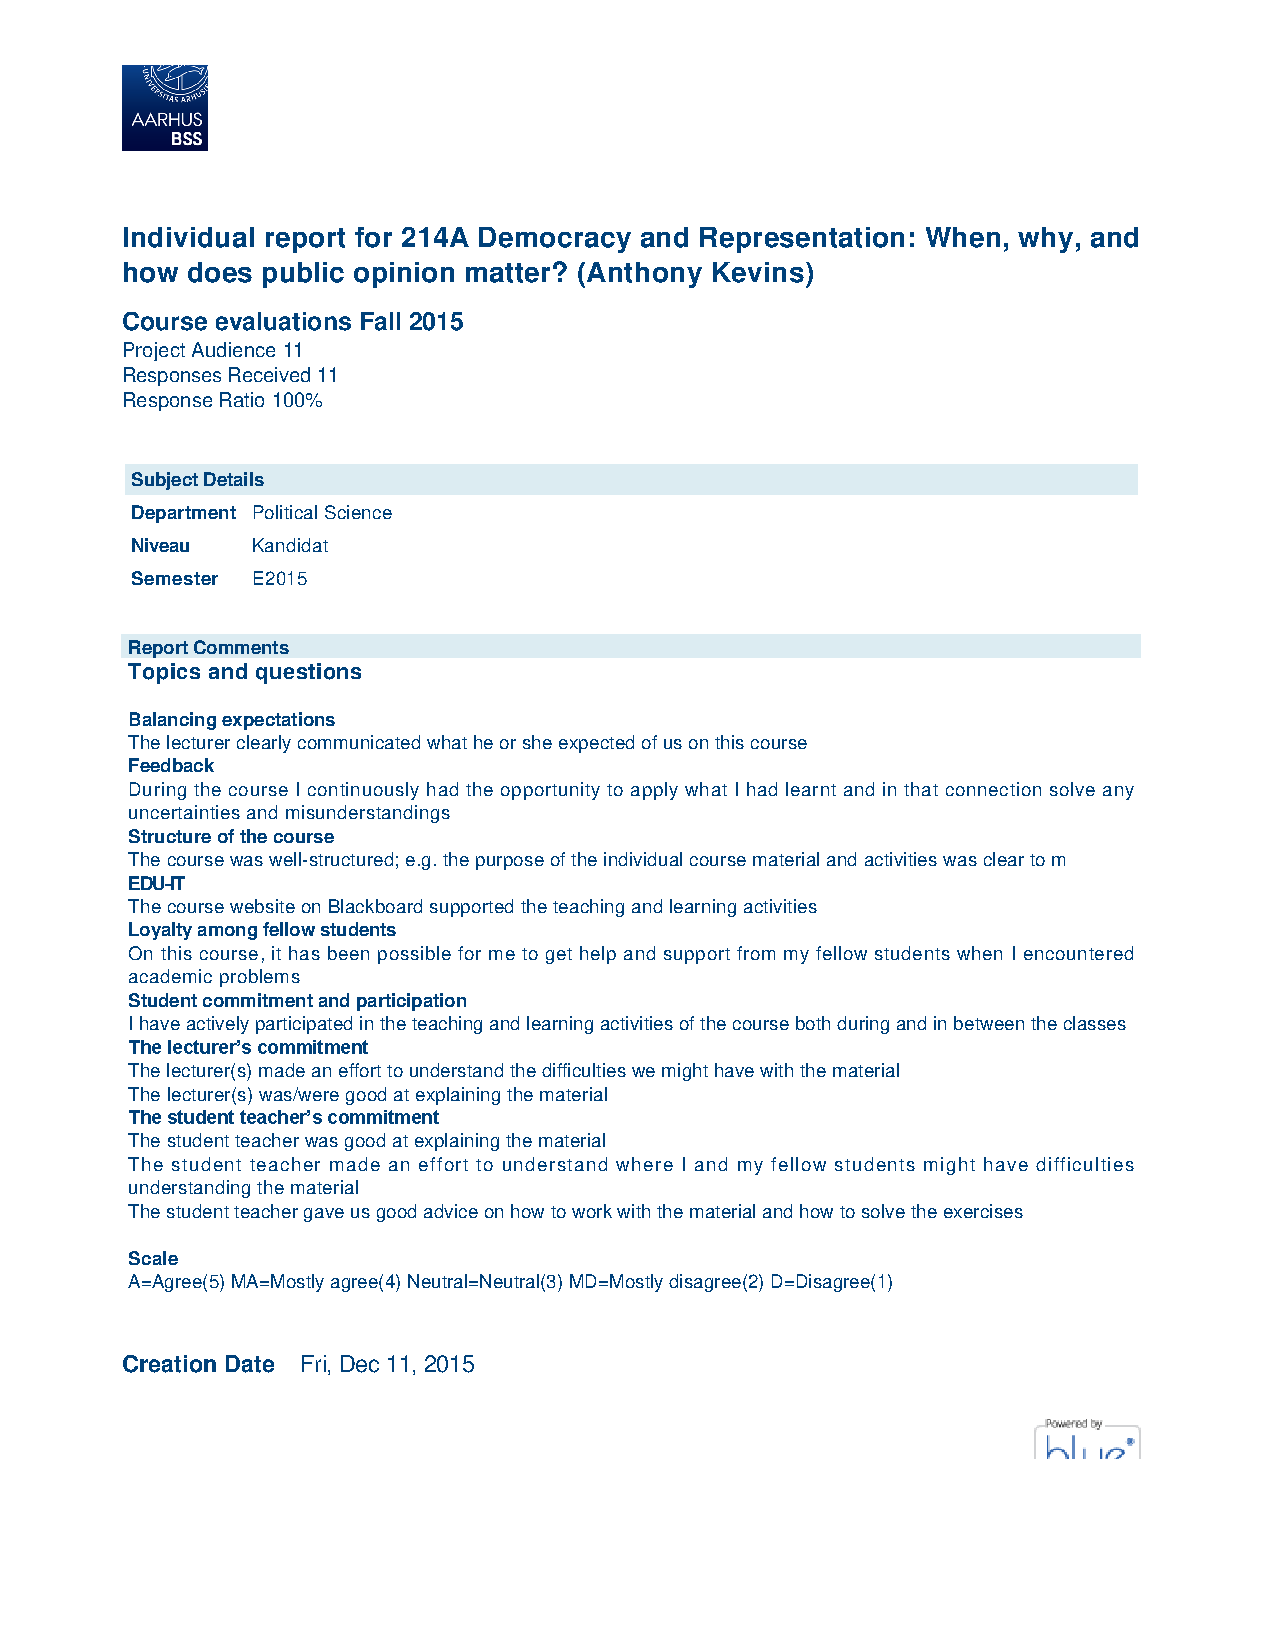
\includepdf[pages=-,pagecommand={\thispagestyle{plain}},width=\textwidth,height=\textheight,keepaspectratio,trim=30pt 30pt 30pt 30pt]{Evaluations2.pdf}

\renewcommand{\headrulewidth}{0pt}

\begin{figure}
Political Institutions, Aarhus University\par\medskip
\thispagestyle{plain}
\centering
\begin{subfigure}{\textwidth}
\includegraphics[page=68,viewport=0 396 612 800,width=\textwidth,clip]%
  {Appendix_Materials.pdf}
\end{subfigure}\\
\begin{subfigure}{\textwidth}
\includegraphics[page=69,viewport=0 396 612 800,width=\textwidth,clip]%
  {Appendix_Materials.pdf}
\end{subfigure}\\
\end{figure}

\newpage

\begin{figure}
Political Institutions, Aarhus University\par\medskip
\thispagestyle{plain}
\centering
\begin{subfigure}{\textwidth}
\includegraphics[page=72,viewport=0 396 612 800,width=\textwidth,clip]%
  {Appendix_Materials.pdf}
\end{subfigure}\\
\begin{subfigure}{\textwidth}
\includegraphics[page=73,viewport=0 396 612 800,width=\textwidth,clip]%
  {Appendix_Materials.pdf}
\end{subfigure}\\
\end{figure}

\end{document}
